% Created by tikzDevice version 0.10.1 on 2016-09-06 08:50:27
% !TEX encoding = UTF-8 Unicode
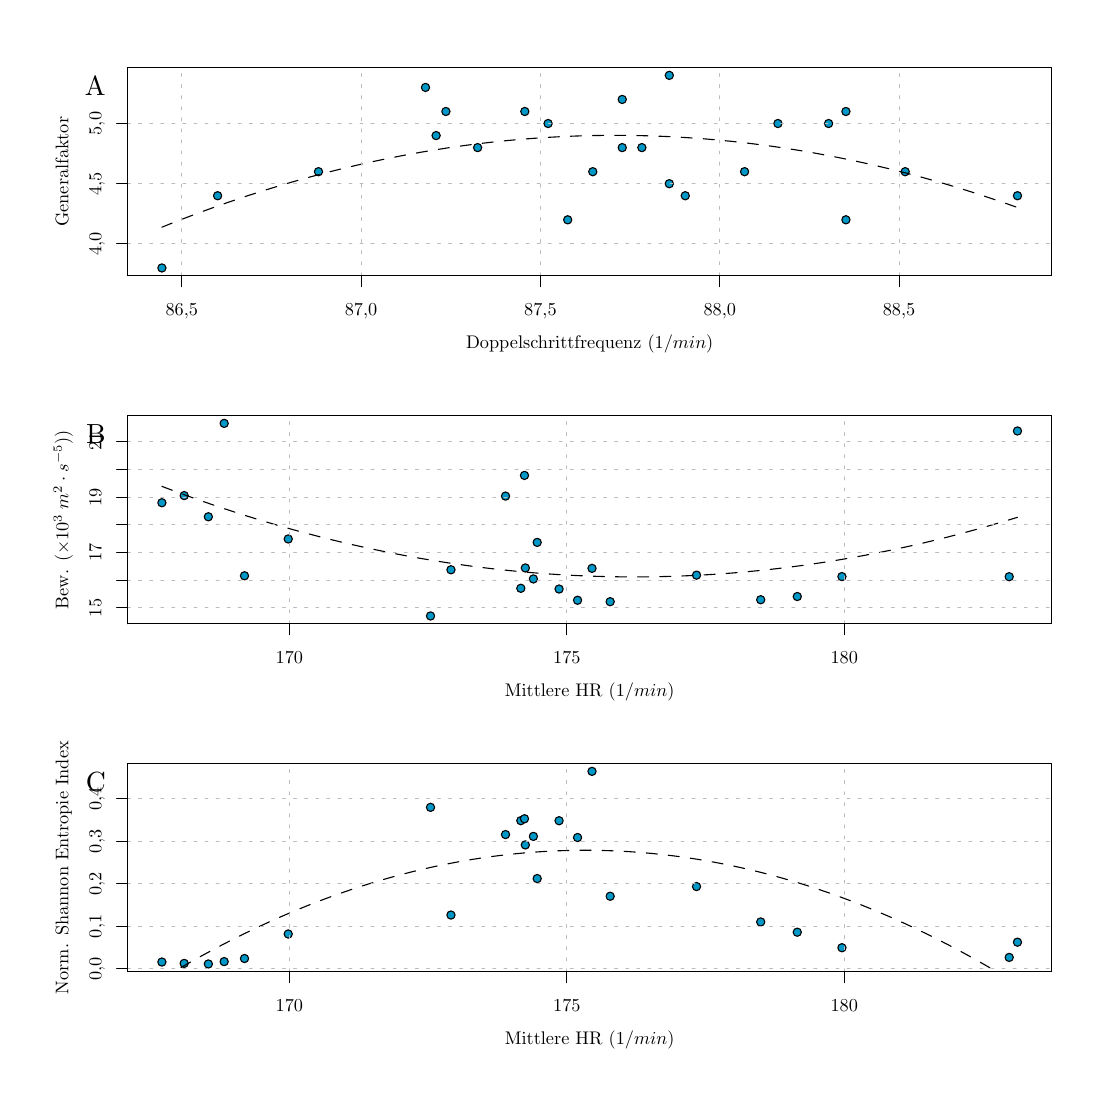
\begin{tikzpicture}[x=1pt,y=1pt]
\definecolor{fillColor}{RGB}{255,255,255}
\path[use as bounding box,fill=fillColor,fill opacity=0.00] (0,0) rectangle (377.25,377.25);
\begin{scope}
\path[clip] ( 36.13,287.63) rectangle (370.02,362.80);
\definecolor{drawColor}{RGB}{0,0,0}
\definecolor{fillColor}{RGB}{0,152,199}

\path[draw=drawColor,line width= 0.4pt,line join=round,line cap=round,fill=fillColor] (259.06,325.21) circle (  1.49);

\path[draw=drawColor,line width= 0.4pt,line join=round,line cap=round,fill=fillColor] (317.09,325.21) circle (  1.49);

\path[draw=drawColor,line width= 0.4pt,line join=round,line cap=round,fill=fillColor] (105.08,325.21) circle (  1.49);

\path[draw=drawColor,line width= 0.4pt,line join=round,line cap=round,fill=fillColor] (231.85,320.87) circle (  1.49);

\path[draw=drawColor,line width= 0.4pt,line join=round,line cap=round,fill=fillColor] (295.66,307.82) circle (  1.49);

\path[draw=drawColor,line width= 0.4pt,line join=round,line cap=round,fill=fillColor] (221.94,333.91) circle (  1.49);

\path[draw=drawColor,line width= 0.4pt,line join=round,line cap=round,fill=fillColor] (162.59,333.91) circle (  1.49);

\path[draw=drawColor,line width= 0.4pt,line join=round,line cap=round,fill=fillColor] (204.20,325.21) circle (  1.49);

\path[draw=drawColor,line width= 0.4pt,line join=round,line cap=round,fill=fillColor] (237.62,316.52) circle (  1.49);

\path[draw=drawColor,line width= 0.4pt,line join=round,line cap=round,fill=fillColor] (195.14,307.82) circle (  1.49);

\path[draw=drawColor,line width= 0.4pt,line join=round,line cap=round,fill=fillColor] ( 48.50,290.42) circle (  1.49);

\path[draw=drawColor,line width= 0.4pt,line join=round,line cap=round,fill=fillColor] ( 68.63,316.52) circle (  1.49);

\path[draw=drawColor,line width= 0.4pt,line join=round,line cap=round,fill=fillColor] (289.41,342.61) circle (  1.49);

\path[draw=drawColor,line width= 0.4pt,line join=round,line cap=round,fill=fillColor] (214.84,333.91) circle (  1.49);

\path[draw=drawColor,line width= 0.4pt,line join=round,line cap=round,fill=fillColor] (214.84,351.31) circle (  1.49);

\path[draw=drawColor,line width= 0.4pt,line join=round,line cap=round,fill=fillColor] (271.10,342.61) circle (  1.49);

\path[draw=drawColor,line width= 0.4pt,line join=round,line cap=round,fill=fillColor] (295.67,346.96) circle (  1.49);

\path[draw=drawColor,line width= 0.4pt,line join=round,line cap=round,fill=fillColor] (147.59,338.26) circle (  1.49);

\path[draw=drawColor,line width= 0.4pt,line join=round,line cap=round,fill=fillColor] (151.12,346.96) circle (  1.49);

\path[draw=drawColor,line width= 0.4pt,line join=round,line cap=round,fill=fillColor] (143.75,355.66) circle (  1.49);

\path[draw=drawColor,line width= 0.4pt,line join=round,line cap=round,fill=fillColor] (231.85,360.01) circle (  1.49);

\path[draw=drawColor,line width= 0.4pt,line join=round,line cap=round,fill=fillColor] (179.64,346.96) circle (  1.49);

\path[draw=drawColor,line width= 0.4pt,line join=round,line cap=round,fill=fillColor] (188.05,342.61) circle (  1.49);

\path[draw=drawColor,line width= 0.4pt,line join=round,line cap=round,fill=fillColor] (357.66,316.52) circle (  1.49);
\end{scope}
\begin{scope}
\path[clip] (  0.00,  0.00) rectangle (377.25,377.25);
\definecolor{drawColor}{RGB}{0,0,0}

\path[draw=drawColor,line width= 0.4pt,line join=round,line cap=round] ( 55.67,287.63) -- (314.89,287.63);

\path[draw=drawColor,line width= 0.4pt,line join=round,line cap=round] ( 55.67,287.63) -- ( 55.67,283.67);

\path[draw=drawColor,line width= 0.4pt,line join=round,line cap=round] (120.48,287.63) -- (120.48,283.67);

\path[draw=drawColor,line width= 0.4pt,line join=round,line cap=round] (185.28,287.63) -- (185.28,283.67);

\path[draw=drawColor,line width= 0.4pt,line join=round,line cap=round] (250.09,287.63) -- (250.09,283.67);

\path[draw=drawColor,line width= 0.4pt,line join=round,line cap=round] (314.89,287.63) -- (314.89,283.67);

\node[text=drawColor,anchor=base,inner sep=0pt, outer sep=0pt, scale=  0.66] at ( 55.67,273.38) {86,5};

\node[text=drawColor,anchor=base,inner sep=0pt, outer sep=0pt, scale=  0.66] at (120.48,273.38) {87,0};

\node[text=drawColor,anchor=base,inner sep=0pt, outer sep=0pt, scale=  0.66] at (185.28,273.38) {87,5};

\node[text=drawColor,anchor=base,inner sep=0pt, outer sep=0pt, scale=  0.66] at (250.09,273.38) {88,0};

\node[text=drawColor,anchor=base,inner sep=0pt, outer sep=0pt, scale=  0.66] at (314.89,273.38) {88,5};

\path[draw=drawColor,line width= 0.4pt,line join=round,line cap=round] ( 36.13,299.12) -- ( 36.13,342.61);

\path[draw=drawColor,line width= 0.4pt,line join=round,line cap=round] ( 36.13,299.12) -- ( 32.17,299.12);

\path[draw=drawColor,line width= 0.4pt,line join=round,line cap=round] ( 36.13,320.87) -- ( 32.17,320.87);

\path[draw=drawColor,line width= 0.4pt,line join=round,line cap=round] ( 36.13,342.61) -- ( 32.17,342.61);

\node[text=drawColor,rotate= 90.00,anchor=base,inner sep=0pt, outer sep=0pt, scale=  0.66] at ( 26.63,299.12) {4,0};

\node[text=drawColor,rotate= 90.00,anchor=base,inner sep=0pt, outer sep=0pt, scale=  0.66] at ( 26.63,320.87) {4,5};

\node[text=drawColor,rotate= 90.00,anchor=base,inner sep=0pt, outer sep=0pt, scale=  0.66] at ( 26.63,342.61) {5,0};

\path[draw=drawColor,line width= 0.4pt,line join=round,line cap=round] ( 36.13,287.63) --
	(370.02,287.63) --
	(370.02,362.80) --
	( 36.13,362.80) --
	( 36.13,287.63);
\end{scope}
\begin{scope}
\path[clip] (  0.00,251.50) rectangle (377.25,377.25);
\definecolor{drawColor}{RGB}{0,0,0}

\node[text=drawColor,anchor=base,inner sep=0pt, outer sep=0pt, scale=  0.66] at (203.08,261.50) {Doppelschrittfrequenz ($1/min$)};

\node[text=drawColor,rotate= 90.00,anchor=base,inner sep=0pt, outer sep=0pt, scale=  0.66] at ( 14.75,325.21) {Generalfaktor};
\end{scope}
\begin{scope}
\path[clip] ( 36.13,287.63) rectangle (370.02,362.80);
\definecolor{drawColor}{RGB}{0,0,0}

\path[draw=drawColor,line width= 0.4pt,dash pattern=on 4pt off 4pt ,line join=round,line cap=round] ( 48.50,305.15) --
	( 51.62,306.40) --
	( 54.75,307.63) --
	( 57.87,308.83) --
	( 60.99,310.01) --
	( 64.12,311.17) --
	( 67.24,312.30) --
	( 70.36,313.41) --
	( 73.48,314.49) --
	( 76.61,315.55) --
	( 79.73,316.59) --
	( 82.85,317.60) --
	( 85.97,318.59) --
	( 89.10,319.55) --
	( 92.22,320.49) --
	( 95.34,321.41) --
	( 98.47,322.30) --
	(101.59,323.17) --
	(104.71,324.01) --
	(107.83,324.83) --
	(110.96,325.62) --
	(114.08,326.40) --
	(117.20,327.14) --
	(120.33,327.87) --
	(123.45,328.56) --
	(126.57,329.24) --
	(129.69,329.89) --
	(132.82,330.51) --
	(135.94,331.12) --
	(139.06,331.69) --
	(142.18,332.25) --
	(145.31,332.78) --
	(148.43,333.28) --
	(151.55,333.77) --
	(154.68,334.22) --
	(157.80,334.66) --
	(160.92,335.07) --
	(164.04,335.45) --
	(167.17,335.81) --
	(170.29,336.15) --
	(173.41,336.46) --
	(176.54,336.75) --
	(179.66,337.02) --
	(182.78,337.26) --
	(185.90,337.47) --
	(189.03,337.67) --
	(192.15,337.83) --
	(195.27,337.98) --
	(198.39,338.10) --
	(201.52,338.19) --
	(204.64,338.27) --
	(207.76,338.31) --
	(210.89,338.34) --
	(214.01,338.34) --
	(217.13,338.31) --
	(220.25,338.26) --
	(223.38,338.19) --
	(226.50,338.09) --
	(229.62,337.97) --
	(232.75,337.83) --
	(235.87,337.66) --
	(238.99,337.46) --
	(242.11,337.25) --
	(245.24,337.01) --
	(248.36,336.74) --
	(251.48,336.45) --
	(254.60,336.14) --
	(257.73,335.80) --
	(260.85,335.44) --
	(263.97,335.05) --
	(267.10,334.64) --
	(270.22,334.21) --
	(273.34,333.75) --
	(276.46,333.26) --
	(279.59,332.76) --
	(282.71,332.23) --
	(285.83,331.67) --
	(288.96,331.09) --
	(292.08,330.49) --
	(295.20,329.86) --
	(298.32,329.21) --
	(301.45,328.54) --
	(304.57,327.84) --
	(307.69,327.11) --
	(310.81,326.37) --
	(313.94,325.59) --
	(317.06,324.80) --
	(320.18,323.98) --
	(323.31,323.13) --
	(326.43,322.26) --
	(329.55,321.37) --
	(332.67,320.46) --
	(335.80,319.52) --
	(338.92,318.55) --
	(342.04,317.56) --
	(345.17,316.55) --
	(348.29,315.51) --
	(351.41,314.45) --
	(354.53,313.37) --
	(357.66,312.26);
\definecolor{drawColor}{RGB}{186,187,194}

\path[draw=drawColor,line width= 0.4pt,dash pattern=on 1pt off 3pt ,line join=round,line cap=round] ( 55.67,287.63) -- ( 55.67,362.80);

\path[draw=drawColor,line width= 0.4pt,dash pattern=on 1pt off 3pt ,line join=round,line cap=round] (120.48,287.63) -- (120.48,362.80);

\path[draw=drawColor,line width= 0.4pt,dash pattern=on 1pt off 3pt ,line join=round,line cap=round] (185.28,287.63) -- (185.28,362.80);

\path[draw=drawColor,line width= 0.4pt,dash pattern=on 1pt off 3pt ,line join=round,line cap=round] (250.09,287.63) -- (250.09,362.80);

\path[draw=drawColor,line width= 0.4pt,dash pattern=on 1pt off 3pt ,line join=round,line cap=round] (314.89,287.63) -- (314.89,362.80);

\path[draw=drawColor,line width= 0.4pt,dash pattern=on 1pt off 3pt ,line join=round,line cap=round] ( 36.14,299.12) -- (370.02,299.12);

\path[draw=drawColor,line width= 0.4pt,dash pattern=on 1pt off 3pt ,line join=round,line cap=round] ( 36.14,320.87) -- (370.02,320.87);

\path[draw=drawColor,line width= 0.4pt,dash pattern=on 1pt off 3pt ,line join=round,line cap=round] ( 36.14,342.61) -- (370.02,342.61);
\end{scope}
\begin{scope}
\path[clip] (  0.00,  0.00) rectangle (377.25,377.25);
\definecolor{drawColor}{RGB}{0,0,0}

\path[draw=drawColor,line width= 0.4pt,line join=round,line cap=round] ( 36.13,287.63) --
	(370.02,287.63) --
	(370.02,362.80) --
	( 36.13,362.80) --
	( 36.13,287.63);

\node[text=drawColor,anchor=base east,inner sep=0pt, outer sep=0pt, scale=  1.00] at ( 28.21,352.76) {A};
\end{scope}
\begin{scope}
\path[clip] ( 36.13,161.88) rectangle (370.02,237.05);
\definecolor{drawColor}{RGB}{0,0,0}
\definecolor{fillColor}{RGB}{0,152,199}

\path[draw=drawColor,line width= 0.4pt,line join=round,line cap=round,fill=fillColor] ( 48.50,205.58) circle (  1.49);

\path[draw=drawColor,line width= 0.4pt,line join=round,line cap=round,fill=fillColor] ( 65.29,200.51) circle (  1.49);

\path[draw=drawColor,line width= 0.4pt,line join=round,line cap=round,fill=fillColor] ( 94.15,192.49) circle (  1.49);

\path[draw=drawColor,line width= 0.4pt,line join=round,line cap=round,fill=fillColor] ( 56.55,208.17) circle (  1.49);

\path[draw=drawColor,line width= 0.4pt,line join=round,line cap=round,fill=fillColor] (184.11,191.25) circle (  1.49);

\path[draw=drawColor,line width= 0.4pt,line join=round,line cap=round,fill=fillColor] (203.92,181.87) circle (  1.49);

\path[draw=drawColor,line width= 0.4pt,line join=round,line cap=round,fill=fillColor] (241.69,179.42) circle (  1.49);

\path[draw=drawColor,line width= 0.4pt,line join=round,line cap=round,fill=fillColor] (182.74,178.05) circle (  1.49);

\path[draw=drawColor,line width= 0.4pt,line join=round,line cap=round,fill=fillColor] (179.83,182.02) circle (  1.49);

\path[draw=drawColor,line width= 0.4pt,line join=round,line cap=round,fill=fillColor] (178.20,174.66) circle (  1.49);

\path[draw=drawColor,line width= 0.4pt,line join=round,line cap=round,fill=fillColor] (145.57,164.67) circle (  1.49);

\path[draw=drawColor,line width= 0.4pt,line join=round,line cap=round,fill=fillColor] (210.48,169.83) circle (  1.49);

\path[draw=drawColor,line width= 0.4pt,line join=round,line cap=round,fill=fillColor] (152.95,181.36) circle (  1.49);

\path[draw=drawColor,line width= 0.4pt,line join=round,line cap=round,fill=fillColor] (198.70,170.35) circle (  1.49);

\path[draw=drawColor,line width= 0.4pt,line join=round,line cap=round,fill=fillColor] (264.88,170.53) circle (  1.49);

\path[draw=drawColor,line width= 0.4pt,line join=round,line cap=round,fill=fillColor] (354.67,178.86) circle (  1.49);

\path[draw=drawColor,line width= 0.4pt,line join=round,line cap=round,fill=fillColor] ( 78.35,179.19) circle (  1.49);

\path[draw=drawColor,line width= 0.4pt,line join=round,line cap=round,fill=fillColor] (192.02,174.40) circle (  1.49);

\path[draw=drawColor,line width= 0.4pt,line join=round,line cap=round,fill=fillColor] (278.09,171.69) circle (  1.49);

\path[draw=drawColor,line width= 0.4pt,line join=round,line cap=round,fill=fillColor] (294.23,178.90) circle (  1.49);

\path[draw=drawColor,line width= 0.4pt,line join=round,line cap=round,fill=fillColor] ( 71.00,234.26) circle (  1.49);

\path[draw=drawColor,line width= 0.4pt,line join=round,line cap=round,fill=fillColor] (179.52,215.46) circle (  1.49);

\path[draw=drawColor,line width= 0.4pt,line join=round,line cap=round,fill=fillColor] (172.67,207.98) circle (  1.49);

\path[draw=drawColor,line width= 0.4pt,line join=round,line cap=round,fill=fillColor] (357.66,231.51) circle (  1.49);
\end{scope}
\begin{scope}
\path[clip] (  0.00,  0.00) rectangle (377.25,377.25);
\definecolor{drawColor}{RGB}{0,0,0}

\path[draw=drawColor,line width= 0.4pt,line join=round,line cap=round] ( 94.56,161.88) -- (295.07,161.88);

\path[draw=drawColor,line width= 0.4pt,line join=round,line cap=round] ( 94.56,161.88) -- ( 94.56,157.92);

\path[draw=drawColor,line width= 0.4pt,line join=round,line cap=round] (194.82,161.88) -- (194.82,157.92);

\path[draw=drawColor,line width= 0.4pt,line join=round,line cap=round] (295.07,161.88) -- (295.07,157.92);

\node[text=drawColor,anchor=base,inner sep=0pt, outer sep=0pt, scale=  0.66] at ( 94.56,147.63) {170};

\node[text=drawColor,anchor=base,inner sep=0pt, outer sep=0pt, scale=  0.66] at (194.82,147.63) {175};

\node[text=drawColor,anchor=base,inner sep=0pt, outer sep=0pt, scale=  0.66] at (295.07,147.63) {180};

\path[draw=drawColor,line width= 0.4pt,line join=round,line cap=round] ( 36.13,167.57) -- ( 36.13,227.66);

\path[draw=drawColor,line width= 0.4pt,line join=round,line cap=round] ( 36.13,167.57) -- ( 32.17,167.57);

\path[draw=drawColor,line width= 0.4pt,line join=round,line cap=round] ( 36.13,177.58) -- ( 32.17,177.58);

\path[draw=drawColor,line width= 0.4pt,line join=round,line cap=round] ( 36.13,187.60) -- ( 32.17,187.60);

\path[draw=drawColor,line width= 0.4pt,line join=round,line cap=round] ( 36.13,197.61) -- ( 32.17,197.61);

\path[draw=drawColor,line width= 0.4pt,line join=round,line cap=round] ( 36.13,207.63) -- ( 32.17,207.63);

\path[draw=drawColor,line width= 0.4pt,line join=round,line cap=round] ( 36.13,217.65) -- ( 32.17,217.65);

\path[draw=drawColor,line width= 0.4pt,line join=round,line cap=round] ( 36.13,227.66) -- ( 32.17,227.66);

\node[text=drawColor,rotate= 90.00,anchor=base,inner sep=0pt, outer sep=0pt, scale=  0.66] at ( 26.63,167.57) {15};

\node[text=drawColor,rotate= 90.00,anchor=base,inner sep=0pt, outer sep=0pt, scale=  0.66] at ( 26.63,187.60) {17};

\node[text=drawColor,rotate= 90.00,anchor=base,inner sep=0pt, outer sep=0pt, scale=  0.66] at ( 26.63,207.63) {19};

\node[text=drawColor,rotate= 90.00,anchor=base,inner sep=0pt, outer sep=0pt, scale=  0.66] at ( 26.63,227.66) {21};

\path[draw=drawColor,line width= 0.4pt,line join=round,line cap=round] ( 36.13,161.88) --
	(370.02,161.88) --
	(370.02,237.05) --
	( 36.13,237.05) --
	( 36.13,161.88);
\end{scope}
\begin{scope}
\path[clip] (  0.00,125.75) rectangle (377.25,251.50);
\definecolor{drawColor}{RGB}{0,0,0}

\node[text=drawColor,anchor=base,inner sep=0pt, outer sep=0pt, scale=  0.66] at (203.08,135.75) {Mittlere HR ($1/min$)};

\node[text=drawColor,rotate= 90.00,anchor=base,inner sep=0pt, outer sep=0pt, scale=  0.66] at ( 14.75,199.47) {Bew. ($\times 10^3 \: m^2 \cdot s^{-5}$))};
\end{scope}
\begin{scope}
\path[clip] ( 36.13,161.88) rectangle (370.02,237.05);
\definecolor{drawColor}{RGB}{0,0,0}

\path[draw=drawColor,line width= 0.4pt,dash pattern=on 4pt off 4pt ,line join=round,line cap=round] ( 48.50,211.50) --
	( 51.62,210.32) --
	( 54.75,209.15) --
	( 57.87,208.01) --
	( 60.99,206.89) --
	( 64.12,205.79) --
	( 67.24,204.72) --
	( 70.36,203.66) --
	( 73.48,202.63) --
	( 76.61,201.62) --
	( 79.73,200.63) --
	( 82.85,199.66) --
	( 85.97,198.71) --
	( 89.10,197.79) --
	( 92.22,196.89) --
	( 95.34,196.01) --
	( 98.47,195.15) --
	(101.59,194.32) --
	(104.71,193.50) --
	(107.83,192.71) --
	(110.96,191.94) --
	(114.08,191.19) --
	(117.20,190.46) --
	(120.33,189.76) --
	(123.45,189.08) --
	(126.57,188.42) --
	(129.69,187.78) --
	(132.82,187.16) --
	(135.94,186.57) --
	(139.06,185.99) --
	(142.18,185.44) --
	(145.31,184.91) --
	(148.43,184.41) --
	(151.55,183.92) --
	(154.68,183.46) --
	(157.80,183.02) --
	(160.92,182.60) --
	(164.04,182.20) --
	(167.17,181.82) --
	(170.29,181.47) --
	(173.41,181.14) --
	(176.54,180.83) --
	(179.66,180.54) --
	(182.78,180.27) --
	(185.90,180.03) --
	(189.03,179.81) --
	(192.15,179.60) --
	(195.27,179.43) --
	(198.39,179.27) --
	(201.52,179.13) --
	(204.64,179.02) --
	(207.76,178.93) --
	(210.89,178.86) --
	(214.01,178.81) --
	(217.13,178.79) --
	(220.25,178.79) --
	(223.38,178.80) --
	(226.50,178.84) --
	(229.62,178.91) --
	(232.75,178.99) --
	(235.87,179.10) --
	(238.99,179.23) --
	(242.11,179.38) --
	(245.24,179.55) --
	(248.36,179.74) --
	(251.48,179.96) --
	(254.60,180.19) --
	(257.73,180.45) --
	(260.85,180.74) --
	(263.97,181.04) --
	(267.10,181.36) --
	(270.22,181.71) --
	(273.34,182.08) --
	(276.46,182.47) --
	(279.59,182.88) --
	(282.71,183.32) --
	(285.83,183.78) --
	(288.96,184.25) --
	(292.08,184.75) --
	(295.20,185.28) --
	(298.32,185.82) --
	(301.45,186.39) --
	(304.57,186.98) --
	(307.69,187.59) --
	(310.81,188.22) --
	(313.94,188.87) --
	(317.06,189.55) --
	(320.18,190.24) --
	(323.31,190.96) --
	(326.43,191.71) --
	(329.55,192.47) --
	(332.67,193.25) --
	(335.80,194.06) --
	(338.92,194.89) --
	(342.04,195.74) --
	(345.17,196.61) --
	(348.29,197.51) --
	(351.41,198.43) --
	(354.53,199.36) --
	(357.66,200.32);
\definecolor{drawColor}{RGB}{186,187,194}

\path[draw=drawColor,line width= 0.4pt,dash pattern=on 1pt off 3pt ,line join=round,line cap=round] ( 94.56,161.88) -- ( 94.56,237.05);

\path[draw=drawColor,line width= 0.4pt,dash pattern=on 1pt off 3pt ,line join=round,line cap=round] (194.82,161.88) -- (194.82,237.05);

\path[draw=drawColor,line width= 0.4pt,dash pattern=on 1pt off 3pt ,line join=round,line cap=round] (295.07,161.88) -- (295.07,237.05);

\path[draw=drawColor,line width= 0.4pt,dash pattern=on 1pt off 3pt ,line join=round,line cap=round] ( 36.13,167.57) -- (370.02,167.57);

\path[draw=drawColor,line width= 0.4pt,dash pattern=on 1pt off 3pt ,line join=round,line cap=round] ( 36.13,177.58) -- (370.02,177.58);

\path[draw=drawColor,line width= 0.4pt,dash pattern=on 1pt off 3pt ,line join=round,line cap=round] ( 36.13,187.60) -- (370.02,187.60);

\path[draw=drawColor,line width= 0.4pt,dash pattern=on 1pt off 3pt ,line join=round,line cap=round] ( 36.13,197.61) -- (370.02,197.61);

\path[draw=drawColor,line width= 0.4pt,dash pattern=on 1pt off 3pt ,line join=round,line cap=round] ( 36.13,207.63) -- (370.02,207.63);

\path[draw=drawColor,line width= 0.4pt,dash pattern=on 1pt off 3pt ,line join=round,line cap=round] ( 36.13,217.65) -- (370.02,217.65);

\path[draw=drawColor,line width= 0.4pt,dash pattern=on 1pt off 3pt ,line join=round,line cap=round] ( 36.13,227.66) -- (370.02,227.66);
\end{scope}
\begin{scope}
\path[clip] (  0.00,  0.00) rectangle (377.25,377.25);
\definecolor{drawColor}{RGB}{0,0,0}

\path[draw=drawColor,line width= 0.4pt,line join=round,line cap=round] ( 36.13,161.88) --
	(370.02,161.88) --
	(370.02,237.05) --
	( 36.13,237.05) --
	( 36.13,161.88);

\node[text=drawColor,anchor=base east,inner sep=0pt, outer sep=0pt, scale=  1.00] at ( 28.21,227.01) {B};
\end{scope}
\begin{scope}
\path[clip] ( 36.13, 36.13) rectangle (370.02,111.30);
\definecolor{drawColor}{RGB}{0,0,0}
\definecolor{fillColor}{RGB}{0,152,199}

\path[draw=drawColor,line width= 0.4pt,line join=round,line cap=round,fill=fillColor] ( 48.50, 39.62) circle (  1.49);

\path[draw=drawColor,line width= 0.4pt,line join=round,line cap=round,fill=fillColor] ( 65.29, 38.92) circle (  1.49);

\path[draw=drawColor,line width= 0.4pt,line join=round,line cap=round,fill=fillColor] ( 94.15, 49.75) circle (  1.49);

\path[draw=drawColor,line width= 0.4pt,line join=round,line cap=round,fill=fillColor] ( 56.55, 39.13) circle (  1.49);

\path[draw=drawColor,line width= 0.4pt,line join=round,line cap=round,fill=fillColor] (184.11, 69.78) circle (  1.49);

\path[draw=drawColor,line width= 0.4pt,line join=round,line cap=round,fill=fillColor] (203.92,108.51) circle (  1.49);

\path[draw=drawColor,line width= 0.4pt,line join=round,line cap=round,fill=fillColor] (241.69, 66.89) circle (  1.49);

\path[draw=drawColor,line width= 0.4pt,line join=round,line cap=round,fill=fillColor] (182.74, 85.02) circle (  1.49);

\path[draw=drawColor,line width= 0.4pt,line join=round,line cap=round,fill=fillColor] (179.83, 81.94) circle (  1.49);

\path[draw=drawColor,line width= 0.4pt,line join=round,line cap=round,fill=fillColor] (178.20, 90.70) circle (  1.49);

\path[draw=drawColor,line width= 0.4pt,line join=round,line cap=round,fill=fillColor] (145.57, 95.52) circle (  1.49);

\path[draw=drawColor,line width= 0.4pt,line join=round,line cap=round,fill=fillColor] (210.48, 63.39) circle (  1.49);

\path[draw=drawColor,line width= 0.4pt,line join=round,line cap=round,fill=fillColor] (152.95, 56.60) circle (  1.49);

\path[draw=drawColor,line width= 0.4pt,line join=round,line cap=round,fill=fillColor] (198.70, 84.61) circle (  1.49);

\path[draw=drawColor,line width= 0.4pt,line join=round,line cap=round,fill=fillColor] (264.88, 54.10) circle (  1.49);

\path[draw=drawColor,line width= 0.4pt,line join=round,line cap=round,fill=fillColor] (354.67, 41.29) circle (  1.49);

\path[draw=drawColor,line width= 0.4pt,line join=round,line cap=round,fill=fillColor] ( 78.35, 40.89) circle (  1.49);

\path[draw=drawColor,line width= 0.4pt,line join=round,line cap=round,fill=fillColor] (192.02, 90.68) circle (  1.49);

\path[draw=drawColor,line width= 0.4pt,line join=round,line cap=round,fill=fillColor] (278.09, 50.40) circle (  1.49);

\path[draw=drawColor,line width= 0.4pt,line join=round,line cap=round,fill=fillColor] (294.23, 44.79) circle (  1.49);

\path[draw=drawColor,line width= 0.4pt,line join=round,line cap=round,fill=fillColor] ( 71.00, 39.77) circle (  1.49);

\path[draw=drawColor,line width= 0.4pt,line join=round,line cap=round,fill=fillColor] (179.52, 91.39) circle (  1.49);

\path[draw=drawColor,line width= 0.4pt,line join=round,line cap=round,fill=fillColor] (172.67, 85.68) circle (  1.49);

\path[draw=drawColor,line width= 0.4pt,line join=round,line cap=round,fill=fillColor] (357.66, 46.79) circle (  1.49);
\end{scope}
\begin{scope}
\path[clip] (  0.00,  0.00) rectangle (377.25,377.25);
\definecolor{drawColor}{RGB}{0,0,0}

\path[draw=drawColor,line width= 0.4pt,line join=round,line cap=round] ( 94.56, 36.13) -- (295.07, 36.13);

\path[draw=drawColor,line width= 0.4pt,line join=round,line cap=round] ( 94.56, 36.13) -- ( 94.56, 32.17);

\path[draw=drawColor,line width= 0.4pt,line join=round,line cap=round] (194.82, 36.13) -- (194.82, 32.17);

\path[draw=drawColor,line width= 0.4pt,line join=round,line cap=round] (295.07, 36.13) -- (295.07, 32.17);

\node[text=drawColor,anchor=base,inner sep=0pt, outer sep=0pt, scale=  0.66] at ( 94.56, 21.88) {170};

\node[text=drawColor,anchor=base,inner sep=0pt, outer sep=0pt, scale=  0.66] at (194.82, 21.88) {175};

\node[text=drawColor,anchor=base,inner sep=0pt, outer sep=0pt, scale=  0.66] at (295.07, 21.88) {180};

\path[draw=drawColor,line width= 0.4pt,line join=round,line cap=round] ( 36.13, 37.14) -- ( 36.13, 98.58);

\path[draw=drawColor,line width= 0.4pt,line join=round,line cap=round] ( 36.13, 37.14) -- ( 32.17, 37.14);

\path[draw=drawColor,line width= 0.4pt,line join=round,line cap=round] ( 36.13, 52.50) -- ( 32.17, 52.50);

\path[draw=drawColor,line width= 0.4pt,line join=round,line cap=round] ( 36.13, 67.86) -- ( 32.17, 67.86);

\path[draw=drawColor,line width= 0.4pt,line join=round,line cap=round] ( 36.13, 83.22) -- ( 32.17, 83.22);

\path[draw=drawColor,line width= 0.4pt,line join=round,line cap=round] ( 36.13, 98.58) -- ( 32.17, 98.58);

\node[text=drawColor,rotate= 90.00,anchor=base,inner sep=0pt, outer sep=0pt, scale=  0.66] at ( 26.63, 37.14) {0,0};

\node[text=drawColor,rotate= 90.00,anchor=base,inner sep=0pt, outer sep=0pt, scale=  0.66] at ( 26.63, 52.50) {0,1};

\node[text=drawColor,rotate= 90.00,anchor=base,inner sep=0pt, outer sep=0pt, scale=  0.66] at ( 26.63, 67.86) {0,2};

\node[text=drawColor,rotate= 90.00,anchor=base,inner sep=0pt, outer sep=0pt, scale=  0.66] at ( 26.63, 83.22) {0,3};

\node[text=drawColor,rotate= 90.00,anchor=base,inner sep=0pt, outer sep=0pt, scale=  0.66] at ( 26.63, 98.58) {0,4};

\path[draw=drawColor,line width= 0.4pt,line join=round,line cap=round] ( 36.13, 36.13) --
	(370.02, 36.13) --
	(370.02,111.30) --
	( 36.13,111.30) --
	( 36.13, 36.13);
\end{scope}
\begin{scope}
\path[clip] (  0.00,  0.00) rectangle (377.25,125.75);
\definecolor{drawColor}{RGB}{0,0,0}

\node[text=drawColor,anchor=base,inner sep=0pt, outer sep=0pt, scale=  0.66] at (203.08, 10.00) {Mittlere HR ($1/min$)};

\node[text=drawColor,rotate= 90.00,anchor=base,inner sep=0pt, outer sep=0pt, scale=  0.66] at ( 14.75, 73.72) {Norm. Shannon Entropie Index};
\end{scope}
\begin{scope}
\path[clip] ( 36.13, 36.13) rectangle (370.02,111.30);
\definecolor{drawColor}{RGB}{0,0,0}

\path[draw=drawColor,line width= 0.4pt,dash pattern=on 4pt off 4pt ,line join=round,line cap=round] ( 48.50, 33.53) --
	( 51.62, 35.41) --
	( 54.75, 37.24) --
	( 57.87, 39.05) --
	( 60.99, 40.81) --
	( 64.12, 42.53) --
	( 67.24, 44.22) --
	( 70.36, 45.86) --
	( 73.48, 47.47) --
	( 76.61, 49.04) --
	( 79.73, 50.57) --
	( 82.85, 52.06) --
	( 85.97, 53.51) --
	( 89.10, 54.92) --
	( 92.22, 56.30) --
	( 95.34, 57.63) --
	( 98.47, 58.93) --
	(101.59, 60.19) --
	(104.71, 61.41) --
	(107.83, 62.59) --
	(110.96, 63.73) --
	(114.08, 64.83) --
	(117.20, 65.90) --
	(120.33, 66.93) --
	(123.45, 67.91) --
	(126.57, 68.86) --
	(129.69, 69.77) --
	(132.82, 70.64) --
	(135.94, 71.47) --
	(139.06, 72.27) --
	(142.18, 73.02) --
	(145.31, 73.74) --
	(148.43, 74.42) --
	(151.55, 75.05) --
	(154.68, 75.65) --
	(157.80, 76.22) --
	(160.92, 76.74) --
	(164.04, 77.22) --
	(167.17, 77.67) --
	(170.29, 78.07) --
	(173.41, 78.44) --
	(176.54, 78.77) --
	(179.66, 79.06) --
	(182.78, 79.31) --
	(185.90, 79.52) --
	(189.03, 79.70) --
	(192.15, 79.83) --
	(195.27, 79.93) --
	(198.39, 79.99) --
	(201.52, 80.01) --
	(204.64, 79.99) --
	(207.76, 79.93) --
	(210.89, 79.83) --
	(214.01, 79.69) --
	(217.13, 79.52) --
	(220.25, 79.31) --
	(223.38, 79.05) --
	(226.50, 78.76) --
	(229.62, 78.43) --
	(232.75, 78.06) --
	(235.87, 77.66) --
	(238.99, 77.21) --
	(242.11, 76.73) --
	(245.24, 76.20) --
	(248.36, 75.64) --
	(251.48, 75.04) --
	(254.60, 74.40) --
	(257.73, 73.72) --
	(260.85, 73.01) --
	(263.97, 72.25) --
	(267.10, 71.46) --
	(270.22, 70.62) --
	(273.34, 69.75) --
	(276.46, 68.84) --
	(279.59, 67.89) --
	(282.71, 66.90) --
	(285.83, 65.87) --
	(288.96, 64.81) --
	(292.08, 63.70) --
	(295.20, 62.56) --
	(298.32, 61.38) --
	(301.45, 60.16) --
	(304.57, 58.90) --
	(307.69, 57.60) --
	(310.81, 56.27) --
	(313.94, 54.89) --
	(317.06, 53.48) --
	(320.18, 52.02) --
	(323.31, 50.53) --
	(326.43, 49.00) --
	(329.55, 47.43) --
	(332.67, 45.82) --
	(335.80, 44.18) --
	(338.92, 42.49) --
	(342.04, 40.77) --
	(345.17, 39.00) --
	(348.29, 37.20) --
	(351.41, 35.36) --
	(354.53, 33.48) --
	(357.66, 31.57);
\definecolor{drawColor}{RGB}{186,187,194}

\path[draw=drawColor,line width= 0.4pt,dash pattern=on 1pt off 3pt ,line join=round,line cap=round] ( 94.56, 36.13) -- ( 94.56,111.30);

\path[draw=drawColor,line width= 0.4pt,dash pattern=on 1pt off 3pt ,line join=round,line cap=round] (194.82, 36.13) -- (194.82,111.30);

\path[draw=drawColor,line width= 0.4pt,dash pattern=on 1pt off 3pt ,line join=round,line cap=round] (295.07, 36.13) -- (295.07,111.30);

\path[draw=drawColor,line width= 0.4pt,dash pattern=on 1pt off 3pt ,line join=round,line cap=round] ( 36.13, 37.14) -- (370.02, 37.14);

\path[draw=drawColor,line width= 0.4pt,dash pattern=on 1pt off 3pt ,line join=round,line cap=round] ( 36.13, 52.50) -- (370.02, 52.50);

\path[draw=drawColor,line width= 0.4pt,dash pattern=on 1pt off 3pt ,line join=round,line cap=round] ( 36.13, 67.86) -- (370.02, 67.86);

\path[draw=drawColor,line width= 0.4pt,dash pattern=on 1pt off 3pt ,line join=round,line cap=round] ( 36.13, 83.22) -- (370.02, 83.22);

\path[draw=drawColor,line width= 0.4pt,dash pattern=on 1pt off 3pt ,line join=round,line cap=round] ( 36.13, 98.58) -- (370.02, 98.58);
\end{scope}
\begin{scope}
\path[clip] (  0.00,  0.00) rectangle (377.25,377.25);
\definecolor{drawColor}{RGB}{0,0,0}

\path[draw=drawColor,line width= 0.4pt,line join=round,line cap=round] ( 36.13, 36.13) --
	(370.02, 36.13) --
	(370.02,111.30) --
	( 36.13,111.30) --
	( 36.13, 36.13);

\node[text=drawColor,anchor=base east,inner sep=0pt, outer sep=0pt, scale=  1.00] at ( 28.21,101.26) {C};
\end{scope}
\end{tikzpicture}
